分组交换可进一步分为\textbf{面向连接的虚电路方式}和\textbf{无连接的数据报方式}。

\textbf{{1.数据报}}\\

如图2-5所示,假设主机A给主机B发送一个报文,高层协议会将报文拆分成若干个带有序号和完整目的地址的分组,交换机根据转发表转发分组。其原理如下:

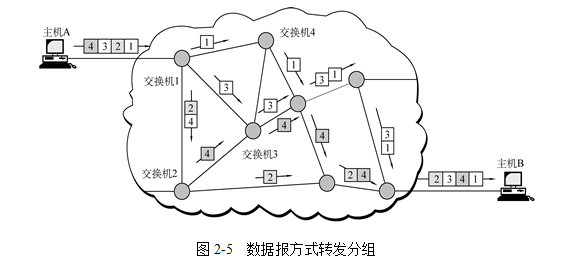
\includegraphics[width=3.92708in,height=1.81250in]{png-jpeg-pics/C224275A3474E63C00208B6761EED1AD.png}

1)首先主机A先将分组逐个地发往与它直接相连的交换机1,交换机1将主机A发来的分组缓存。

2)然后查找自己的转发表,不同时刻转发表的内容可能不相同,因此有的分组转发给交换机2,有的分组转发给交换机3和交换机4。

3)依次类推,直到所有分组到达主机B。

由以上分析可知\textbf{数据报方式具有以下特点:}

1)\textbf{无需建立连接;}

2)\textbf{网络尽最大努力交付,传输不保证可靠性;}

3)\textbf{减小了延迟,大大提高吞吐量;}

4)\textbf{对故障适应能力强;}

5)\textbf{不独占某一链路},\textbf{资源利用率高}。

\textbf{{2.虚电路}}

虚电路方式要求在发送数据之前,\textbf{在源主机和目的主机之间建立一条虚连接}。一旦虚连接建立以后,用户发送的数据(以分组为单位)将通过该路径按顺序传送到达目的主机。当通信完成之后用户发出释放虚电路请求,由网络清除该虚连接。

以上描述是不是有一种似曾相识的感觉?没错,\textbf{虚电路方式与电路交换方式极其相似。其实虚电路方式就是将数据报方式与电路交换方式结合起来},充分发挥二者优点。由以上分析可知,虚电路方式的通信过程分为3个阶段:\textbf{虚电路建立、数据传输与虚电路释放阶段}。

如图2-6和图2-7所示,假设主机A给主机B发送一个报文,原理如下:

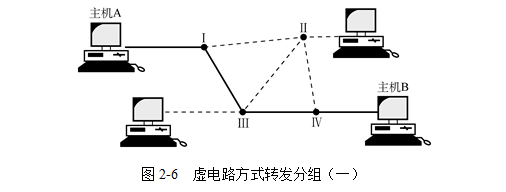
\includegraphics[width=3.18750in,height=1.20833in]{png-jpeg-pics/D2FBE3A39101979D224FC209707A4654.png}

1)主机A先发出一个特殊的``呼叫请求''分组,该分组通过中间交换机(图2-6中的小圆点)送往主机B。如果同意连接,主机B就发送``呼叫应答''分组进行确认,虚电路就建立好了。

2)虚电路建立之后,主机A就可以向主机B发送分组了。由于所有分组都是走同样的路径,因此分组一定按序到达目的主机。

3)分组传输结束后,主机通过发送``释放请求''分组以拆除虚电路,整个连接就断开了。\\
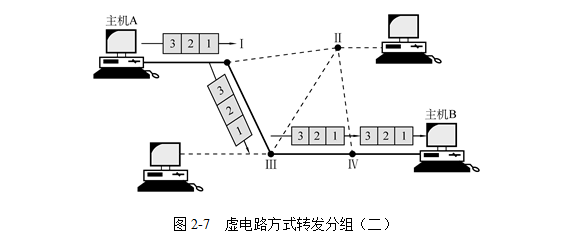
\includegraphics[width=3.90625in,height=1.65625in]{png-jpeg-pics/D4D6AC5E1F36D4650BC26427C569970B.png}

由以上分析可知\textbf{虚电路方式具有以下特点:}

1)\textbf{通信必须建立连接;}\\
2)分组\textbf{按序到达目的主机;}\\
3)\textbf{开销小;}\\
4)当某个交换机或链路出现故障,所有虚电路将遭到破坏。

{\textbf{{3.数据报服务与虚电路服务比较}}}

见表2-2。

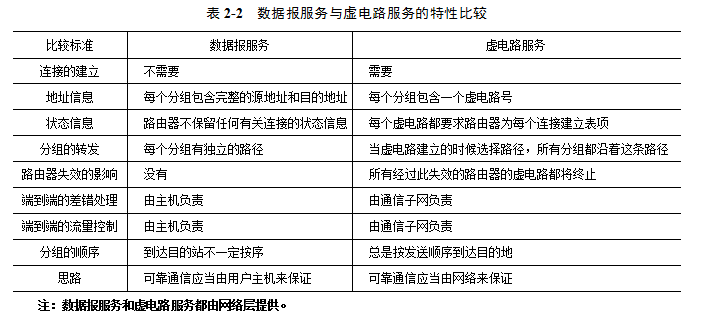
\includegraphics[width=3.37500in,height=1.56250in]{png-jpeg-pics/C10B967B07F6EA214328B987CE4557D1.png}
